% THIS IS SIGPROC-SP.TEX - VERSION 3.1
% WORKS WITH V3.2SP OF ACM_PROC_ARTICLE-SP.CLS
% APRIL 2009
%
% It is an example file showing how to use the 'acm_proc_article-sp.cls' V3.2SP
% LaTeX2e document class file for Conference Proceedings submissions.
% ----------------------------------------------------------------------------------------------------------------
% This .tex file (and associated .cls V3.2SP) *DOES NOT* produce:
%       1) The Permission Statement
%       2) The Conference (location) Info information
%       3) The Copyright Line with ACM data
%       4) Page numbering
% ---------------------------------------------------------------------------------------------------------------
% It is an example which *does* use the .bib file (from which the .bbl file
% is produced).
% REMEMBER HOWEVER: After having produced the .bbl file,
% and prior to final submission,
% you need to 'insert'  your .bbl file into your source .tex file so as to provide
% ONE 'self-contained' source file.
%
% Questions regarding SIGS should be sent to
% Adrienne Griscti ---> griscti@acm.org
%
% Questions/suggestions regarding the guidelines, .tex and .cls files, etc. to
% Gerald Murray ---> murray@hq.acm.org
%
% For tracking purposes - this is V3.1SP - APRIL 2009

\documentclass{acm_proc_article-sp}

\usepackage[linesnumbered, ruled, vlined]{algorithm2e}
\usepackage{subfigure}
\usepackage{graphicx}

\newcommand\mb\mathbf

\begin{document}

\title{Large-scale Image Labeling via Mapreduce Topic Modeling}
\subtitle{[Spring 2012 CMSC828G Final Project Report]
\titlenote{Data-Intensive Computing with MapReduce}}

\numberofauthors{3} %  in this sample file, there are a *total*
% of EIGHT authors. SIX appear on the 'first-page' (for formatting
% reasons) and the remaining two appear in the \additionalauthors section.
%
\author{
% You can go ahead and credit any number of authors here,
% e.g. one 'row of three' or two rows (consisting of one row of three
% and a second row of one, two or three).
%
% The command \alignauthor (no curly braces needed) should
% precede each author name, affiliation/snail-mail address and
% e-mail address. Additionally, tag each line of
% affiliation/address with \affaddr, and tag the
% e-mail address with \email.
%
% 1st. author
\alignauthor
Khoa Doan\\
       \affaddr{University of Maryland}\\
       \affaddr{Dept. of Computer Science}\\
       \affaddr{College Park, MD 20742}\\
       \email{trovato@corporation.com}
%% 2nd. author
\alignauthor
Rahmatri Mardiko\\
       \affaddr{University of Maryland}\\
       \affaddr{Dept. of Computer Science}\\
       \affaddr{College Park, MD 20742}\\
       \email{mardiko@cs.umd.edu}
%% 3rd. author
\alignauthor 
Ang Li\\
       \affaddr{University of Maryland}\\
       \affaddr{Dept. of Computer Science}\\
       \affaddr{College Park, MD}\\
       \email{angli@cs.umd.edu}
}
% There's nothing stopping you putting the seventh, eighth, etc.
% author on the opening page (as the 'third row') but we ask,
% for aesthetic reasons that you place these 'additional authors'
% in the \additional authors block, viz.

\date{\today}
% Just remember to make sure that the TOTAL number of authors
% is the number that will appear on the first page PLUS the
% number that will appear in the \additionalauthors section.

\maketitle
\begin{abstract}
Large scale computer vision is recently being popular due to the emerging of large scale imagery data and in need of more generally trained visual models.
Recent advances in feature extraction provide a feasible and succinct way to represent image regions. However, most of these features are computationally heavy to extract. Since there is no explicit method to essentially speed up feature extraction, parallelization becomes the most comfortable strategy for this task.
Due to the inherent high dimensionality of visual data, extracted features can be very noisy and thus not representative for images. Feature quantization is introduced to group similar features into the same low level semantics. K-means clustering is one of the usual choices for quantization while it may suffer from either time or space problems in ordinary environment. Latent Dirichlet Allocation is one of the techniques to discover higher level topic semantics for the context, which was popular in natural language processing. In this project, we unearth the potential of adapting computer vision tasks such as low level feature extraction and higher level image understanding into the MapReduce framework for large scale image dataset. We adopt the MapReduce LDA (Mr.LDA) to find topics across the images and discuss its possible extensions with respect to the image domain.

\end{abstract}

% A category with the (minimum) three required fields
%\category{}{Computer Vision}{Miscellaneous}
%A category including the fourth, optional field follows...
%\category{}{Map}{Metrics}[complexity measures, performance measures]

%\terms{System}

\keywords{Topic modeling, image labeling, parallelization, MapReduce framework} % NOT required for Proceedings

\section{Introduction}
Large scale visual data analysis and machine learning have been recently received much attention during the past few years. Traditional computer vision research focuses on small datasets of images or videos which makes the generalization of these methods difficult. In the current world of big data, a lot of imagery data have been present in the Internet. How to make use of the large scale of data to explore a better visual model has been one of the central problems in the current community. However, one natural problem arised from this task is heavy computational load. Computer vision tasks are usually involved with feature engineering which requires a lot of time and space for experiments. Fortunately, the MapReduce framework provides a reliable approach to large scale data processing.

In this work, we explore the potentials of using MapReduce framework for a standard computer vision task i.e. image labeling. The objective of the image labeling task is to find underlying semantics for each of the image pixels and to find groups of pixels that belong to the same object or semantic. Image labeling has been investigated for decades, although the scale of the dataset is limited due to computational issues. However, the demand of large scale image labeling turns out to be more and more clear in the recent years. One of the reasons is that people are being aware of using computer techniques to assist human annotation for specific imagery data such as remote sensing data. Millions of satellite images are generated for every day and the task of understanding these data is never feasible for human to do exhaustively. The automatic way will benefit the community tremendously in different areas such as surveillance, city planning, national defense, etc.

The rest of this paper is organized as follows.
Section \ref{sec:overview} briefly introduces the system structure of this project.
MapReduce framework for visual feature extraction is discussed in section \ref{sec:feature}.
Details of Mr.LDA is introduced in section \ref{sec:mrlda}. In section \ref{sec:impl}, a few implementation details are
discussed. Section \ref{sec:exp} shows the evaluation methods and experimental results for this project. Discussion on
possible extensions from LDA to Spatial LDA is presented in section \ref{sec:slda}. Finally, the paper concludes in section \ref{sec:con}.


\section{System Overview}\label{sec:overview}

\section{Feature Extraction}\label{sec:feature}
Feature extraction often dominates the most computational resources in computer vision tasks. In this section, we introduce a MapReduce based framework to extract visual features efficiently which distributes the computation loads for raw feature extraction and scales up the construction of feature codebook via MapReduce K-means clustering.
\subsection{Scale Invariant Feature Transform (SIFT)}
In this work, the Scale Invariant Feature Transform (SIFT) \cite{sift} is adopted to describe local regions across the images. Generally, a SIFT descriptor represent a region bounded by a rectangular box centered at $(x_c,y_c)$. The bounding box is uniformly divided into $K\times K$ parts. The gradients are computed in these sub-regions and the gradient magnitudes in $N_b$ (the number of bins) discretized orientations  are computed. A histogram is then constructed to represent the distribution of the gradient magnitudes. Therefore, for each region, the SIFT descriptor is a $K^2N_b$ dimensional histogram vector.

One of the advantages of SIFT descriptors is its invariance to image rotation and translation, which makes this feature very popular among the computer vision community. We base our project on the MPI-CBG JavaSIFT library\cite{mpicbg}.
\subsection{Dense Sampling SIFT Features}
In order to apply SIFT features to represent the whole image for the task of image labeling, each of the pixels ideally should be described. Due to the fact that a neighborhood of pixels usually have little difference and belong to the same semantics, we sample series of small rectangular regions with a parameter \textsc{stepsize} densely across each of the image and compute the SIFT description for each of the regions. The \textsc{stepsize} controls the number of pixels between two consecutive centers of bounding boxes. Thereafter, each image can be converted from visual data to a list of \textsc{(key,value)} pairs where the \textsc{key} is the index $(g_i,x_i,y_i)$ of the regions and the \textsc{value} is the SIFT feature vector $f_i$. $g_i$ is the id of the image that contains the $i$-th region and $(x_i,y_i)$ is the center location of the $i$-th region.

\subsection{Image Input Aggregation}
Given a large number of image files as input, there are several ways of loading them into a MapReduce job. One possible way is creating a text file containing a list of file names and let the mapper reads the files from HDFS and processes them while the reducer does nothing. An alternative way is similar to the first except the reading and processing is moved to the reducer while the mapper just passes the (key,value) pairs. Both are relatively simple and easy to implement. However, due to the small-files problem in Hadoop\cite{smallfiles}, neither the first and the second approach achieves the best performance in terms of processing speed. 

Since Hadoop framework works best with large files, we need to aggregate the images in the dataset into a few big files. This step allows us to speed-up the feature extraction (and other images processing tasks) given a large number of image files as input. We adopt the approach presented in\cite{combinefiles} which creates a MapReduce job that packs multiple files into a \texttt{SequenceFile}. This aggregation is performed as a preprocessing step for the other jobs that take images as input.

\subsection{MapReduce-based Feature Extraction}
A list of image paths is generated in order to locate the image files. Each of the paths is assigned a number as image ID. The MapReduce job takes the path list as input and output sequence files containing region indices as keys and SIFT feature descriptors as values.
\begin{algorithm}[!htb]
\SetAlgoVlined
\SetKwFor{Class}{class}{}{}
\SetKwFor{Method}{method}{}{}
\SetKwFunction{Split}{split}
\SetKwFunction{Map}{map}
\SetKwFunction{Reduce}{reduce}
\SetKwFunction{Emit}{emit }
\SetKwFunction{Readimage}{readImageFromHDFS}
\SetKwFunction{Extract}{extractFeature}
\Class{\sc Mapper}{
\Method{\Map{\FuncSty{LongWritable} key, \FuncSty{Text} value}}{
(\ArgSty{id}, \ArgSty{path}) = \Split{value}\;
\Emit{id, path}
}
}
\Class{\sc Reducer}{
\Method{\Reduce{\FuncSty{IntWritable} key, \FuncSty{Text} value}}{
\ArgSty{id} = \ArgSty{key}\;
\ArgSty{image} = \Readimage{value}\;
\ArgSty{feature} = \Extract{image}\;
\Emit{id, feature}
}
}
\caption{Mapreduce based Visual Feature Extraction}
\end{algorithm}

% \begin{algorithm}[!htb]
% \caption{Mapreduce Feature Extraction}
% \begin{algorithmic}
% \rm
% \Function{mapper}{LongWritable \texttt{key}, Text \texttt{value}}
% \State (\texttt{id}, \texttt{path}) = \textsc{Split}(\texttt{value}, \texttt{'\char`\\t'});
% \State \textbf{emit} (\texttt{id}, \texttt{path});
% \EndFunction
% \end{algorithmic}
% \vskip 1em
% \begin{algorithmic}
% \rm
% \Function{reducer}{IntWritable \texttt{key}, Text \texttt{value}}
% \State \texttt{id} = \texttt{key};
% \State \texttt{image} = \textsc{ReadImageFromHDFS}(\texttt{value});
% \State \texttt{feature} = \textsc{ExtractDenseSIFT}(\texttt{image});
% \State \textbf{emit} (\texttt{id}, \texttt{feature});
% \EndFunction
% \end{algorithmic}
% \end{algorithm}

\subsection{Building Feature Codebook}
The raw features extracted from above generally have two problems in representing the images. On the one hand, the dimension of each feature vector is typically 128. For the similarity measure of each pair of small regions, at least 128 times of multiplications are necessary for Euclidean distances. This makes the further processing intractable even using parallelization framework. On the other hand, the feature vector is a histogram of oriented gradients which contains a lot of noises. Therefore, feature quantization is introduced to further processing the features and construct a "codebook" for the features. In the codebook, nearby feature vectors are grouped into the same index because they should belong to the same visual semantics.

K-means clustering is usually the choice for doing feature quantization. However, the clustering takes more features and thus needs much more memory spaces in order to exhaustively compute the distances between cluster centers to each of the points, as the scale of data becomes larger. The MapReduce framework generally resolve this time and space problem because not only the computation is distributed into different nodes but also the intermediate results of distances are stored almost uniformly among all of the nodes. In our project, we adopt Mahout K-means clustering \cite{mahout} for building the codebook in Hadoop environment.
\section{MapReduce LDA}\label{sec:mrlda}
\cite{mrlda}

\section{MapReduce Spatial LDA}
%\begin{equation}
%\begin{split}
%q(\phi,\pi,d,z &| \lambda,\gamma,\eta,\varphi) = \\
%&\prod\limits_{k=1}^{K}q(\phi_k|\lambda) \: \prod\limits_{m=1}^{M}q(\pi_m|\gamma) \: \prod\limits_{n=1}^{N}q(d_n | \eta) q(z_n | \varphi)
%\end{split}
%\end{equation}
%where $\phi_k \in R^V$ is distribution over word of topic $k$, $\pi_m \in R^K$ is distribution over topics of document $m$, $d_n \in R^M$ is indicator vector where if $d_{nm} = 1$ means word $n$ belongs to document $m$, and $z_n \in R^K$ is indicator vector where if $z_{nk} = 1$ means word $n$ is assigned to topic $k$.

\section{Implementation Remarks}\label{sec:impl}
In this section we present some implementation details that we did in the project.
\subsection{Image-to-SequenceFile Conversion}
In the evaluation phase of the project we need to compare the LDA output and the true labels. To enable pixel-by-pixel evaluation we extract each pixel in the ground truth images and store them as (key,value) pairs. The key, which contains the image id and the pixel position ($x$,$y$), is of type \texttt{TripleOfInts} whereas the value is of type \texttt{IntWritable} and it contains the pixel value. This images-to-pixels conversion can actually be performed as map-only MapReduce job. However, sometimes it is useful to group pixels that have the same semantic together. Here we can apply value-to-key conversion so the pixels that have the same labels are grouped together when they arrive at the reducer.

\begin{algorithm}[!htb]
\SetAlgoVlined
\SetKwFor{Class}{class}{}{}
\SetKwFor{Method}{method}{}{}
\SetKwFunction{Split}{split}
\SetKwFunction{Map}{map}
\SetKwFunction{Reduce}{reduce}
\SetKwFunction{Emit}{emit }
\SetKwFunction{Readimage}{readImageFromHDFS}
\SetKwFunction{Extract}{extractFeature}
\SetKwFunction{Read}{readImageFromBytes}
\SetKwFunction{Size}{sizeOf}
\SetKwFunction{Getpixel}{getPixel}
\SetKwFunction{Iterator}{iterator}
\SetKwFunction{Triple}{triple}
\SetKwFunction{HasNext}{hasNext}
\SetKwFunction{Iterator}{iterator}
\SetKwFunction{Next}{next}
\SetKwFor{Forall}{for all}{do}{}

\Class{\sc Mapper}{
\Method{\Map{\FuncSty{IntWritable} {key}, \FuncSty{BytesWritable} {value}}}{
\ArgSty{image} = \Read{value}\;
(\ArgSty{width}, \ArgSty{height}) = \Size{image}\;
\For{$y = 1 \to$~\ArgSty{height}}{
\For{$x = 1 \to$~\ArgSty{width}}{
\ArgSty{pixel} = \Getpixel{image, x, y}\;
\Emit{pixel, \Triple{key, x, y}}\;
}
}
}
}
\Class{\sc Reducer}{
\Method{\Reduce{\FuncSty{IntWritable} key, \FuncSty{Iterable<TripleOfInts>} value}}{
\ArgSty{iter} = \ArgSty{values}.\Iterator{}\;
\While{\ArgSty{iter}.\HasNext{}}{
\Emit{iter.\Next{}, {key}}\;
}
}
}
\caption{Conversion from Images to SequenceFiles}
\end{algorithm}

% \begin{algorithm}[!htb]
% \caption{MapReduce Convert Images to Pixels}
% \begin{algorithmic}
% \rm
% \Function{mapper}{IntWritable \texttt{key}, BytesWritable \texttt{value}}
% \State \texttt{image} = \textbf{read}(\texttt{value});
% \State \texttt{width,height} = size(\texttt{image});
% \For{$y = 1 \to \texttt{height}$}
% \For{$x = 1 \to \texttt{width}$}
% \State \texttt{pixel} = \textbf{getpixel}\texttt{(image,x,y)};
% \State \textbf{emit} (\texttt{pixel}, \texttt{(key,x,y)});
% \EndFor
% \EndFor
% \EndFunction
% \end{algorithmic}
% \vskip 1em
% \begin{algorithmic}
% \rm
% \Function{reducer}{IntWritable \texttt{key}, Iterable<TripleOfInts> \texttt{values}}
% \State \texttt{iter} = \textbf{iterator}(\texttt{values})
% \While{\texttt{iter.hasNext()}}
% \State \textbf{emit} (\texttt{iter.next()}, \texttt{key});
% \EndWhile
% \EndFunction
% \end{algorithmic}
% \end{algorithm}

\subsection{Sequencefile-to-Image Conversion}
Also for the evaluation purpose, we need to build images from a set of pixels. This task is the inverse of the previous task. The mapper takes ((image\_id,x,y),pixel) pairs and produce (image\_id,(x,y,pixel)) as intermediate key value pairs so the pixels that belong to the same image are grouped together in the reducer. In the reducer the pixels are used to build the image object and convert it to \texttt{BytesWritable}. Since the output is in the form of \texttt{SequenceFile}, we still need to read the output separately to get the individual image files.

\begin{algorithm}[!htb]
\SetAlgoVlined
\SetKwFor{Class}{class}{}{}
\SetKwFor{Method}{method}{}{}
\SetKwFunction{Split}{split}
\SetKwFunction{Map}{map}
\SetKwFunction{Reduce}{reduce}
\SetKwFunction{Emit}{emit }
\SetKwFunction{Readimage}{readImageFromHDFS}
\SetKwFunction{Extract}{extractFeature}
\SetKwFunction{Read}{readImageFromBytes}
\SetKwFunction{Size}{sizeOf}
\SetKwFunction{Getpixel}{getPixel}
\SetKwFunction{Setpixel}{setPixel}
\SetKwFunction{Iterator}{iterator}
\SetKwFunction{Triple}{triple}
\SetKwFunction{HasNext}{hasNext}
\SetKwFunction{Iterator}{iterator}
\SetKwFunction{Next}{next}
\SetKwFunction{GetMembers}{getMembers}
\SetKwFunction{GetBytes}{getBytes}
\SetKwFunction{Image}{image}
\SetKwFor{Forall}{for all}{do}{}

\Class{\sc Mapper}{
\Method{\Map{\FuncSty{TripleOfInts} {key}, \FuncSty{IntWritable} {value}}}{
(\ArgSty{id}, \ArgSty{x}, \ArgSty{y}) = \GetMembers{key}\;
\Emit{id, \Triple{x, y, value}}\;
}
}
\Class{\sc Reducer}{
\Method{\Reduce{\FuncSty{IntWritable} key, \FuncSty{Iterable<TripleOfInts>} value}}{
\ArgSty{image} = \KwSty{new} \Image{width,height}\;
\ArgSty{iter} = \ArgSty{values}.\Iterator{}\;
\While{\ArgSty{iter}.\HasNext{}}{
(\ArgSty{x}, \ArgSty{y}, \ArgSty{pixel}) = \GetMembers{value}\;
\Setpixel{image, x, y, pixel}\;
}

\ArgSty{bytes} = \GetBytes{image}\;
\Emit{key, bytes}\;
}
}
\caption{Conversion from SequenceFiles to Images}
\end{algorithm}
% \begin{algorithm}[!htb]
% \caption{MapReduce Convert Pixels to Images}
% \begin{algorithmic}
% \rm
% \Function{mapper}{TripleOfInts \texttt{key}, IntWritable \texttt{value}}
% \State \texttt{image\_id,x,y} = getmembers(\texttt{key});
% \State \textbf{emit} (\texttt{image\_id}, \texttt{(x,y,value)});
% \EndFunction
% \end{algorithmic}
% \vskip 1em
% \begin{algorithmic}
% \rm
% \Function{reducer}{IntWritable \texttt{key}, Iterable<TripleOfInts> \texttt{values}}
% \State \texttt{image} = \textbf{new image}(\texttt{width,height});
% \State \texttt{iter} = \textbf{iterator}(\texttt{values})
% \While{\texttt{iter.hasNext()}}
% \State \texttt{x,y,pixel} = \textbf{getmembers}(\texttt{value});
% \State \textbf{setpixel}(\texttt{image,x,y,pixel});
% \EndWhile
% 
% \State \texttt{imseq} = \textbf{getbytes}(\texttt{image});
% \State \textbf{emit} (\texttt{key}, imseq);
% \EndFunction
% \end{algorithmic}
% \end{algorithm}

\section{Experimental Evaluation}\label{sec:exp}
\subsection{Dataset}
\subsubsection{MSRC Image Labeling Dataset}
The MSRC image labeling dataset (version 1) \cite{msrc} contains 240 images and 9 object classes in total. 
Each of the images is pixel-wise labeled. Fig.(\ref{fig:msrc}) shows some sample images from MSRC dataset.
\begin{figure}[!htb]
\centering
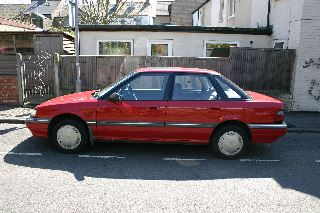
\includegraphics[width=0.11\textwidth]{fig/sample-msrc1}
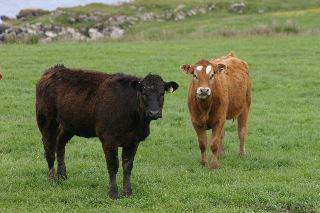
\includegraphics[width=0.11\textwidth]{fig/sample-msrc2}
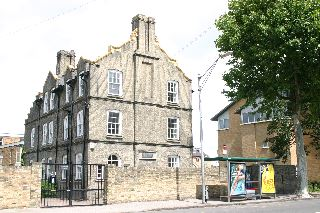
\includegraphics[width=0.11\textwidth]{fig/sample-msrc3}
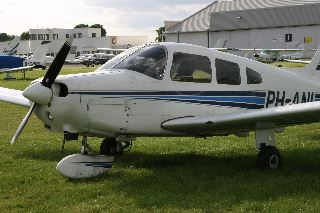
\includegraphics[width=0.11\textwidth]{fig/sample-msrc4}
\caption{Sample images from MSRC Image Labeling Dataset}\label{fig:msrc}
\end{figure}
\subsubsection{Eastern Coast Satellite Image Dataset}
We also collect satellite images using Google Maps APIs along the eastern coast in the United States. Each of the image is of 8-bit colormap PNG format and contains $402\times415$ pixels. Due to the capacity of our cluster, we pick 10,000 images amongst the dataset for the experiments. Fig.(\ref{fig:gmaps}) shows some sample images from Satellite image dataset.
\begin{figure}[!htb]
\centering
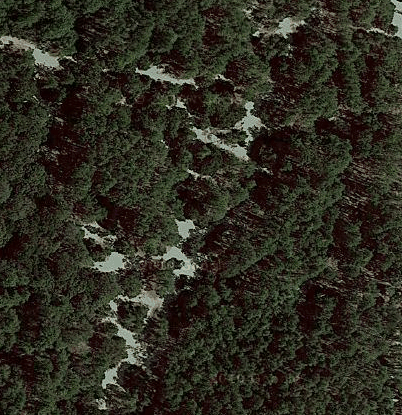
\includegraphics[width=0.11\textwidth]{fig/sample-gmaps1}
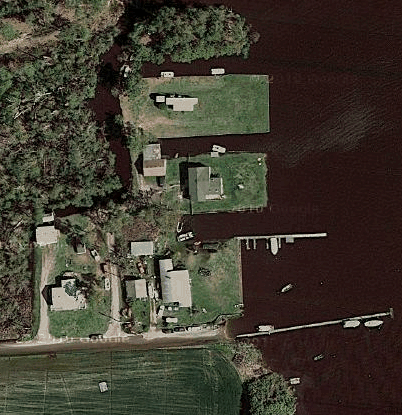
\includegraphics[width=0.11\textwidth]{fig/sample-gmaps2}
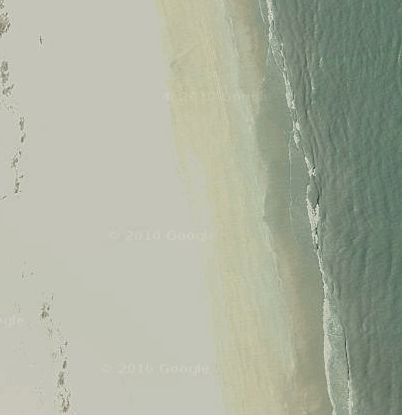
\includegraphics[width=0.11\textwidth]{fig/sample-gmaps3}
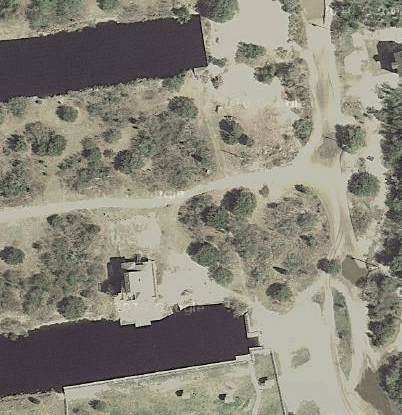
\includegraphics[width=0.11\textwidth]{fig/sample-gmaps4}
\caption{Sample images from Eastern Coast Satellite Image Dataset}\label{fig:gmaps}
\end{figure}

\subsection{Qualitative Evaluation}
Images with labels in different colors are recovered from the output of LDA to show qualitatively which parts belong to the same semantics. Figure \ref{fig:qual} presents three sample images and the output labels with 9 and 14 topics. The ground truth consists of 14 distinct semantics. However, the performance of LDA is significantly higher with 9 topics than 14 topics.
\begin{figure}[!htb]
\centering
\subfigure[origin]{\parbox{0.11\textwidth}{
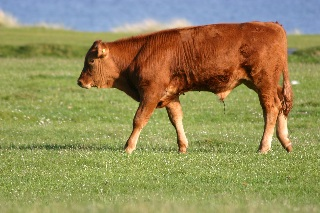
\includegraphics[width=0.11\textwidth]{fig/125-origin}
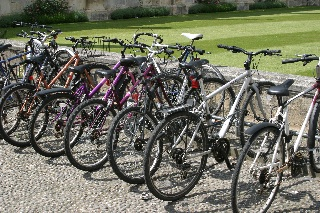
\includegraphics[width=0.11\textwidth]{fig/216-origin}
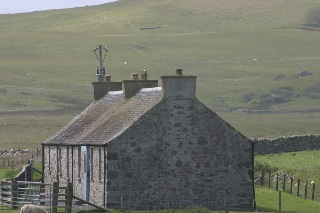
\includegraphics[width=0.11\textwidth]{fig/65-origin}}
}\subfigure[14 topics]{\parbox{0.11\textwidth}{
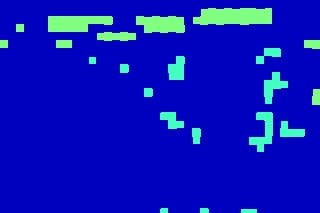
\includegraphics[width=0.11\textwidth]{fig/125-lda-topic14}
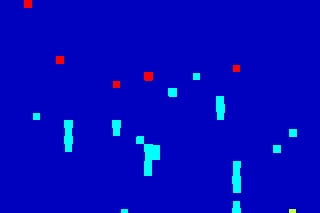
\includegraphics[width=0.11\textwidth]{fig/216-lda-topic14}
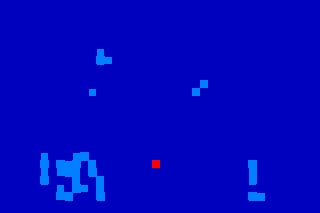
\includegraphics[width=0.11\textwidth]{fig/65-lda-topic14}}
}\subfigure[9 topics]{\parbox{0.11\textwidth}{
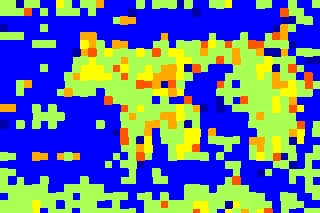
\includegraphics[width=0.11\textwidth]{fig/125-lda-topic9}
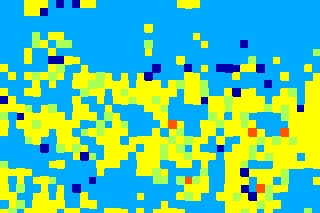
\includegraphics[width=0.11\textwidth]{fig/216-lda-topic9}
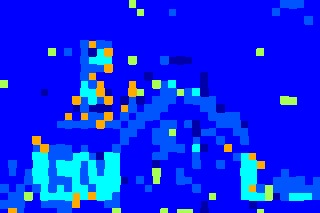
\includegraphics[width=0.11\textwidth]{fig/65-lda-topic9}}
}\subfigure[truth]{\parbox{0.11\textwidth}{
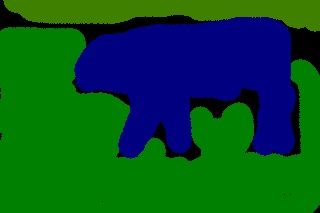
\includegraphics[width=0.11\textwidth]{fig/125-GT}
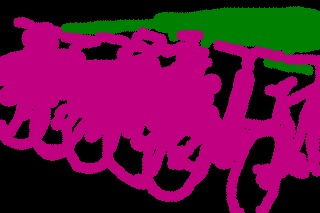
\includegraphics[width=0.11\textwidth]{fig/216-GT}
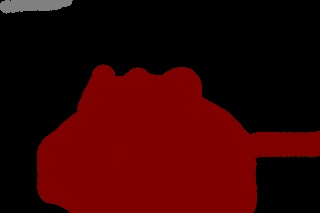
\includegraphics[width=0.11\textwidth]{fig/65-GT}}
}
\caption{Sample LDA output from MSRC dataset. The second and the third column show the output of labeling with LDA using 14 and 9 topics. The last column show the ground truth images.}\label{fig:qual}
\end{figure}

\begin{figure*}
 \centering
 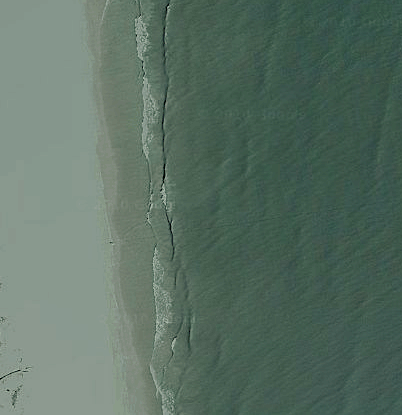
\includegraphics[width=0.1\textwidth]{fig/gmaps/71}
 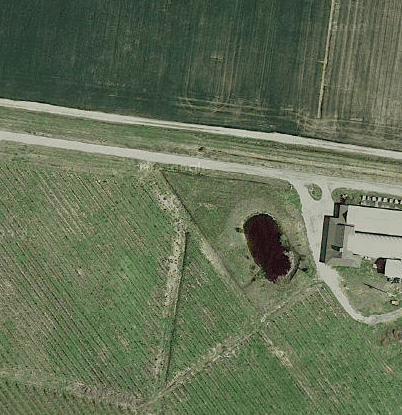
\includegraphics[width=0.1\textwidth]{fig/gmaps/720}
 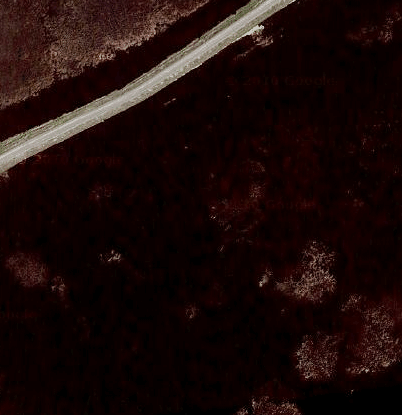
\includegraphics[width=0.1\textwidth]{fig/gmaps/978}
 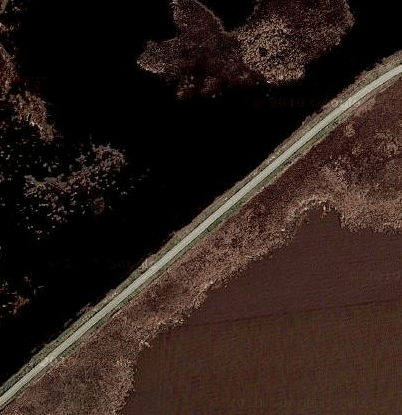
\includegraphics[width=0.1\textwidth]{fig/gmaps/1307}
 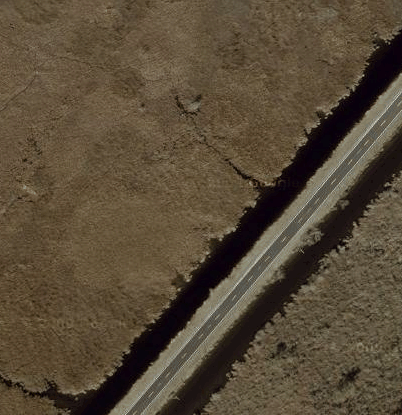
\includegraphics[width=0.1\textwidth]{fig/gmaps/5474}
 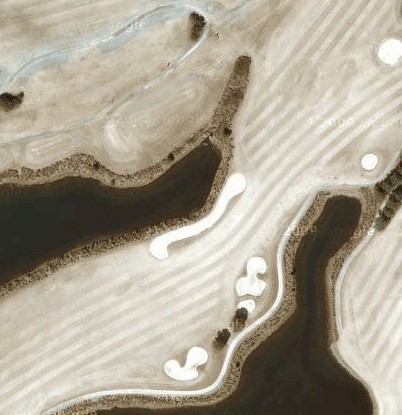
\includegraphics[width=0.1\textwidth]{fig/gmaps/8436}
 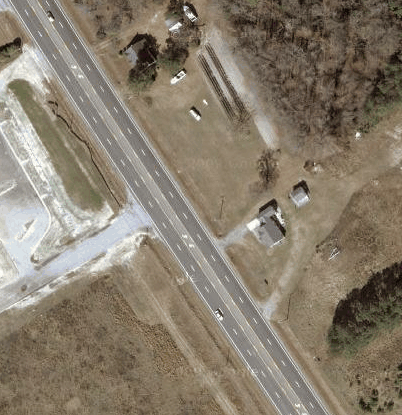
\includegraphics[width=0.1\textwidth]{fig/gmaps/12338}
 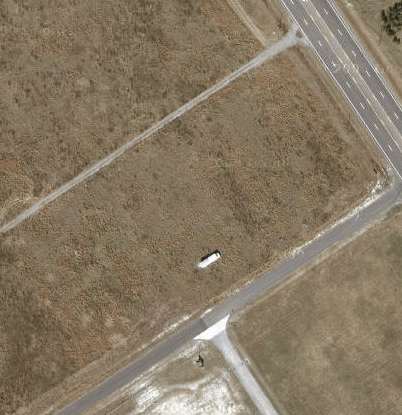
\includegraphics[width=0.1\textwidth]{fig/gmaps/12396}
 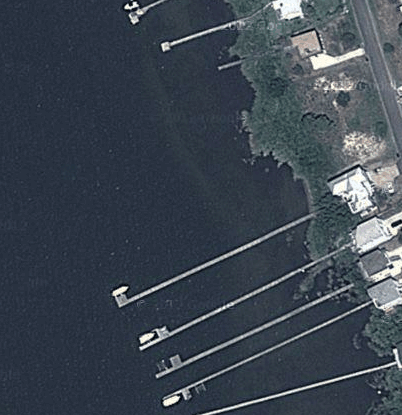
\includegraphics[width=0.1\textwidth]{fig/gmaps/14811}\\
  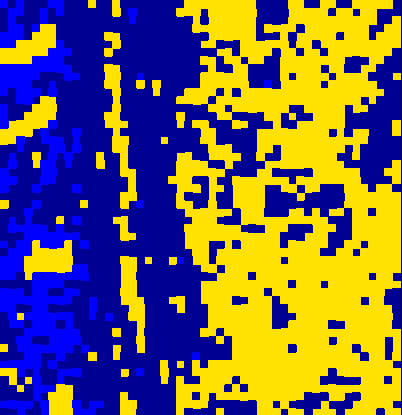
\includegraphics[width=0.1\textwidth]{fig/gmaps/71g}
 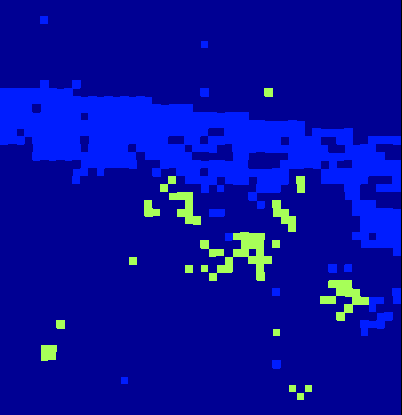
\includegraphics[width=0.1\textwidth]{fig/gmaps/720g}
 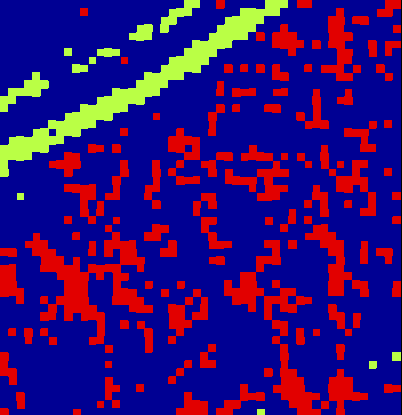
\includegraphics[width=0.1\textwidth]{fig/gmaps/978g}
 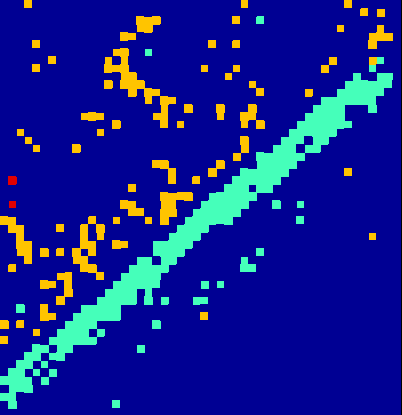
\includegraphics[width=0.1\textwidth]{fig/gmaps/1307g}
 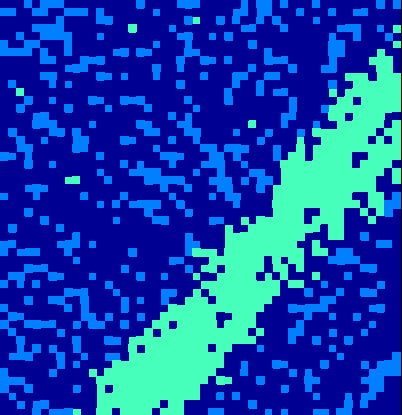
\includegraphics[width=0.1\textwidth]{fig/gmaps/5474g}
 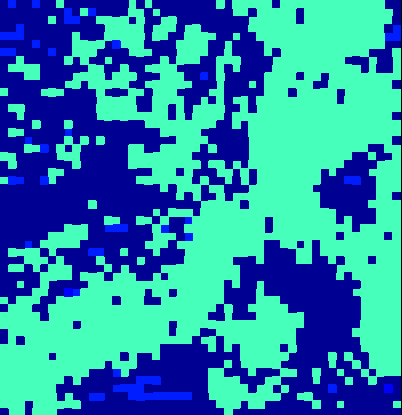
\includegraphics[width=0.1\textwidth]{fig/gmaps/8436g}
 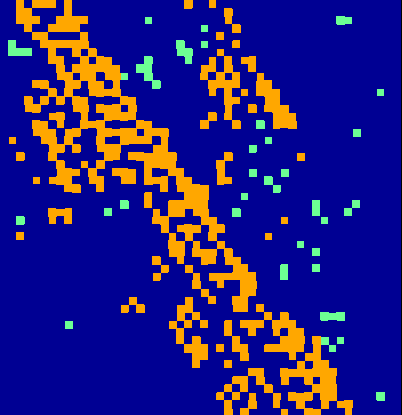
\includegraphics[width=0.1\textwidth]{fig/gmaps/12338g}
 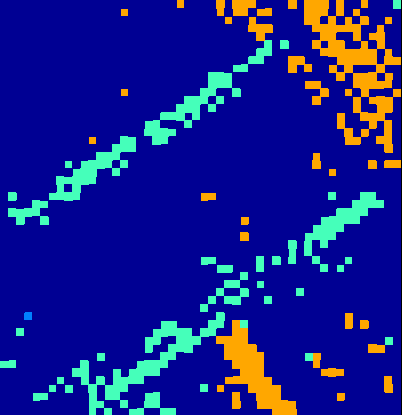
\includegraphics[width=0.1\textwidth]{fig/gmaps/12396g}
 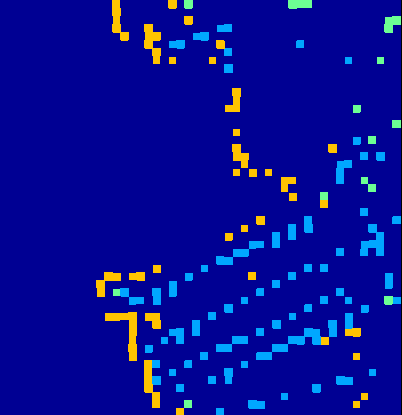
\includegraphics[width=0.1\textwidth]{fig/gmaps/14811g}
 \caption{Qualitative results for Google Maps Satellite Image Dataset}
\end{figure*}


\subsection{Quantitative Evaluation}
Traditional computer vision dataset has ground-truth for evaluation. For the MSRC image labeling data, each image is corresponded to a groundtruth image in which the whole image is divided into several components. Each component is annotated using a unique RGB color. In our output, each pixel is assigned to a type of semantics. Since our approach is completely unsupervised, the truth meaning of each semantic is not understandable. One possible way to evaluate the performance is to enumerate every possible correspondence between the two set of semantics. Apparently this strategy only works when the number of topics is small enough. It becomes difficult to construct a one-one correspondence between our labels and the groundtruth labels. In fact, how to accurately evaluate the performance of image segmentation tasks is still an open problem.

In this project, we propose to evaluate the results for each of the topics separately. For each semantic in the ground truth, a binary image can be constructed, regions with value 1 are those containing such semantic and otherwise not. For the output of the resulted topics, the topic that has the most number of occurrences in the semantic regions are chosen as a correspondence. The precision and recall are then computed according to that topic. Suppose the ground truth is $G:\mb{x}(id,x,y)\to\{1,2,\ldots,K\}$ and the labeling map is $P: \mb{x}(id,x,y)\to\{1,2,\ldots,K'\}$, then the evaluation score for each class $k$ can be computed as
\begin{align}
\text{DetectionRate}(k)&=\frac{\text{cardinal}\left(\{\mb{x}\mid P(\mb{x})=k\}\right)}{\text{cardinal}(\{\mb{x}\mid G(\mb{x})=k\})}\\
\text{FalseAlarm}(k)&=\frac{\text{cardinal}(\{\mb{x}\mid G(\mb{x})\not=k\})}{\text{cardinal}(\{ \mb{x}\mid P(\mb{x})=k\})}
\end{align}
where $\text{cardinal}(\cdot)$ denotes the size of the set.

\begin{figure}[!htb]
 \centering
 \subfigure[9 topics]{
 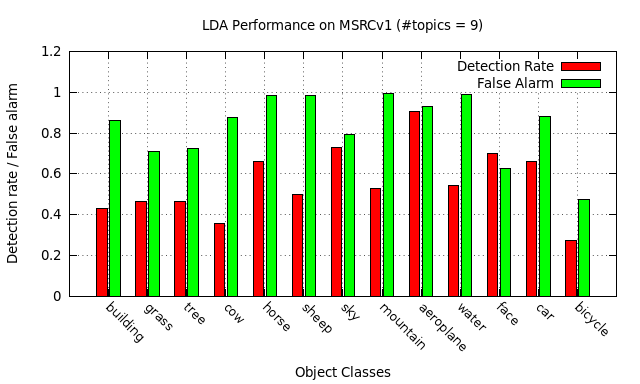
\includegraphics[width=0.45\textwidth]{fig/msrc-quantitative-topic-9}
 }\\\subfigure[14 topics]{
 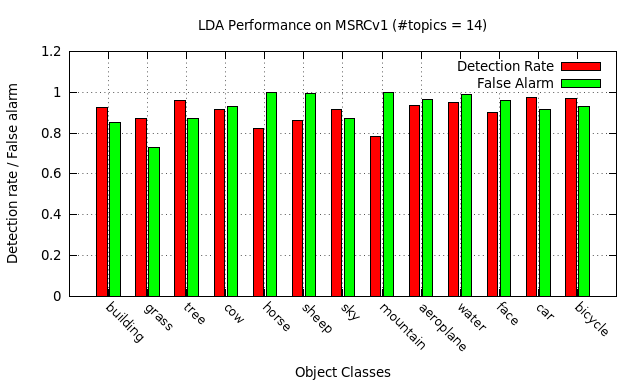
\includegraphics[width=0.45\textwidth]{fig/msrc-quantitative-topic-14}
 }
 \caption{Quantitative evaluation for each classes}
\end{figure}

\section{Discussion: Spatial Latent Dirichlet Allocation}\label{sec:slda}

\section{Conclusion}\label{sec:con}

\section*{Acknowledgments}
The authors would like to thank Prof. Jordan Boyd-Graber and Prof. Jimmy Lin for their consistent help in this project.

\bibliographystyle{abbrv}
\bibliography{sigproc}  % sigproc.bib is the name of the Bibliography in this case

\appendix



\subsubsection{Display Equations}
A numbered display equation -- one set off by vertical space
from the text and centered horizontally -- is produced
by the \textbf{equation} environment. An unnumbered display
equation is produced by the \textbf{displaymath} environment.

Again, in either environment, you can use any of the symbols
and structures available in \LaTeX; this section will just
give a couple of examples of display equations in context.
First, consider the equation, shown as an inline equation above:
\begin{equation}\lim_{n\rightarrow \infty}x=0\end{equation}
Notice how it is formatted somewhat differently in
the \textbf{displaymath}
environment.  Now, we'll enter an unnumbered equation:
\begin{displaymath}\sum_{i=0}^{\infty} x + 1\end{displaymath}
and follow it with another numbered equation:
\begin{equation}\sum_{i=0}^{\infty}x_i=\int_{0}^{\pi+2} f\end{equation}
just to demonstrate \LaTeX's able handling of numbering.

\subsection{Citations}
Citations to articles \cite{bowman:reasoning, clark:pct, braams:babel, herlihy:methodology},
conference
proceedings \cite{clark:pct} or books \cite{salas:calculus, Lamport:LaTeX} listed
in the Bibliography section of your
article will occur throughout the text of your article.
You should use BibTeX to automatically produce this bibliography;
you simply need to insert one of several citation commands with
a key of the item cited in the proper location in
the \texttt{.tex} file \cite{Lamport:LaTeX}.
The key is a short reference you invent to uniquely
identify each work; in this sample document, the key is
the first author's surname and a
word from the title.  This identifying key is included
with each item in the \texttt{.bib} file for your article.

The details of the construction of the \texttt{.bib} file
are beyond the scope of this sample document, but more
information can be found in the \textit{Author's Guide},
and exhaustive details in the \textit{\LaTeX\ User's
Guide}\cite{Lamport:LaTeX}.

This article shows only the plainest form
of the citation command, using \texttt{{\char'134}cite}.
This is what is stipulated in the SIGS style specifications.
No other citation format is endorsed.

\subsection{Tables}
Because tables cannot be split across pages, the best
placement for them is typically the top of the page
nearest their initial cite.  To
ensure this proper ``floating'' placement of tables, use the
environment \textbf{table} to enclose the table's contents and
the table caption.  The contents of the table itself must go
in the \textbf{tabular} environment, to
be aligned properly in rows and columns, with the desired
horizontal and vertical rules.  Again, detailed instructions
on \textbf{tabular} material
is found in the \textit{\LaTeX\ User's Guide}.

Immediately following this sentence is the point at which
Table 1 is included in the input file; compare the
placement of the table here with the table in the printed
dvi output of this document.

\begin{table}
\centering
\caption{Frequency of Special Characters}
\begin{tabular}{|c|c|l|} \hline
Non-English or Math&Frequency&Comments\\ \hline
\O & 1 in 1,000& For Swedish names\\ \hline
$\pi$ & 1 in 5& Common in math\\ \hline
\$ & 4 in 5 & Used in business\\ \hline
$\Psi^2_1$ & 1 in 40,000& Unexplained usage\\
\hline\end{tabular}
\end{table}

To set a wider table, which takes up the whole width of
the page's live area, use the environment
\textbf{table*} to enclose the table's contents and
the table caption.  As with a single-column table, this wide
table will ``float" to a location deemed more desirable.
Immediately following this sentence is the point at which
Table 2 is included in the input file; again, it is
instructive to compare the placement of the
table here with the table in the printed dvi
output of this document.


\begin{table*}
\centering
\caption{Some Typical Commands}
\begin{tabular}{|c|c|l|} \hline
Command&A Number&Comments\\ \hline
\texttt{{\char'134}alignauthor} & 100& Author alignment\\ \hline
\texttt{{\char'134}numberofauthors}& 200& Author enumeration\\ \hline
\texttt{{\char'134}table}& 300 & For tables\\ \hline
\texttt{{\char'134}table*}& 400& For wider tables\\ \hline\end{tabular}
\end{table*}
% end the environment with {table*}, NOTE not {table}!

\subsection{Figures}
Like tables, figures cannot be split across pages; the
best placement for them
is typically the top or the bottom of the page nearest
their initial cite.  To ensure this proper ``floating'' placement
of figures, use the environment
\textbf{figure} to enclose the figure and its caption.

This sample document contains examples of \textbf{.eps}
and \textbf{.ps} files to be displayable with \LaTeX.  More
details on each of these is found in the \textit{Author's Guide}.

\begin{figure}
\centering
\caption{A sample black and white graphic (.eps format).}
\end{figure}

\begin{figure}
\centering
\caption{A sample black and white graphic (.eps format)
that has been resized with the \texttt{epsfig} command.}
\end{figure}


As was the case with tables, you may want a figure
that spans two columns.  To do this, and still to
ensure proper ``floating'' placement of tables, use the environment
\textbf{figure*} to enclose the figure and its caption.

Note that either {\textbf{.ps}} or {\textbf{.eps}} formats are
used; use
the \texttt{{\char'134}epsfig} or \texttt{{\char'134}psfig}
commands as appropriate for the different file types.

\subsection{Theorem-like Constructs}
Other common constructs that may occur in your article are
the forms for logical constructs like theorems, axioms,
corollaries and proofs.  There are
two forms, one produced by the
command \texttt{{\char'134}newtheorem} and the
other by the command \texttt{{\char'134}newdef}; perhaps
the clearest and easiest way to distinguish them is
to compare the two in the output of this sample document:

This uses the \textbf{theorem} environment, created by
the\linebreak\texttt{{\char'134}newtheorem} command:
\newtheorem{theorem}{Theorem}
\begin{theorem}
Let $f$ be continuous on $[a,b]$.  If $G$ is
an antiderivative for $f$ on $[a,b]$, then
\begin{displaymath}\int^b_af(t)dt = G(b) - G(a).\end{displaymath}
\end{theorem}

The other uses the \textbf{definition} environment, created
by the \texttt{{\char'134}newdef} command:
\newdef{definition}{Definition}
\begin{definition}
If $z$ is irrational, then by $e^z$ we mean the
unique number which has
logarithm $z$: \begin{displaymath}{\log e^z = z}\end{displaymath}
\end{definition}

\begin{figure}
\centering
\caption{A sample black and white graphic (.ps format) that has
been resized with the \texttt{psfig} command.}
\end{figure}

Two lists of constructs that use one of these
forms is given in the
\textit{Author's  Guidelines}.

\begin{figure*}
\centering
\caption{A sample black and white graphic (.eps format)
that needs to span two columns of text.}
\end{figure*}
and don't forget to end the environment with
{figure*}, not {figure}!
 
There is one other similar construct environment, which is
already set up
for you; i.e. you must \textit{not} use
a \texttt{{\char'134}newdef} command to
create it: the \textbf{proof} environment.  Here
is a example of its use:
\begin{proof}
Suppose on the contrary there exists a real number $L$ such that
\begin{displaymath}
\lim_{x\rightarrow\infty} \frac{f(x)}{g(x)} = L.
\end{displaymath}
Then
\begin{displaymath}
l=\lim_{x\rightarrow c} f(x)
= \lim_{x\rightarrow c}
\left[ g{x} \cdot \frac{f(x)}{g(x)} \right ]
= \lim_{x\rightarrow c} g(x) \cdot \lim_{x\rightarrow c}
\frac{f(x)}{g(x)} = 0\cdot L = 0,
\end{displaymath}
which contradicts our assumption that $l\neq 0$.
\end{proof}

Complete rules about using these environments and using the
two different creation commands are in the
\textit{Author's Guide}; please consult it for more
detailed instructions.  If you need to use another construct,
not listed therein, which you want to have the same
formatting as the Theorem
or the Definition\cite{salas:calculus} shown above,
use the \texttt{{\char'134}newtheorem} or the
\texttt{{\char'134}newdef} command,
respectively, to create it.

\subsection*{A {\secit Caveat} for the \TeX\ Expert}
Because you have just been given permission to
use the \texttt{{\char'134}newdef} command to create a
new form, you might think you can
use \TeX's \texttt{{\char'134}def} to create a
new command: \textit{Please refrain from doing this!}
Remember that your \LaTeX\ source code is primarily intended
to create camera-ready copy, but may be converted
to other forms -- e.g. HTML. If you inadvertently omit
some or all of the \texttt{{\char'134}def}s recompilation will
be, to say the least, problematic.

\section{Conclusions}
This paragraph will end the body of this sample document.
Remember that you might still have Acknowledgments or
Appendices; brief samples of these
follow.  There is still the Bibliography to deal with; and
we will make a disclaimer about that here: with the exception
of the reference to the \LaTeX\ book, the citations in
this paper are to articles which have nothing to
do with the present subject and are used as
examples only.
%\end{document}  % This is where a 'short' article might terminate

%ACKNOWLEDGMENTS are optional
\section{Acknowledgments}
This section is optional; it is a location for you
to acknowledge grants, funding, editing assistance and
what have you.  In the present case, for example, the
authors would like to thank Gerald Murray of ACM for
his help in codifying this \textit{Author's Guide}
and the \textbf{.cls} and \textbf{.tex} files that it describes.

%
% The following two commands are all you need in the
% initial runs of your .tex file to
% produce the bibliography for the citations in your paper.
% \bibliographystyle{abbrv}
% \bibliography{sigproc}  % sigproc.bib is the name of the Bibliography in this case
% You must have a proper ".bib" file
%  and remember to run:
% latex bibtex latex latex
% to resolve all references
%
% ACM needs 'a single self-contained file'!
%
%APPENDICES are optional
%\balancecolumns
\appendix
%Appendix A
\section{Headings in Appendices}
The rules about hierarchical headings discussed above for
the body of the article are different in the appendices.
In the \textbf{appendix} environment, the command
\textbf{section} is used to
indicate the start of each Appendix, with alphabetic order
designation (i.e. the first is A, the second B, etc.) and
a title (if you include one).  So, if you need
hierarchical structure
\textit{within} an Appendix, start with \textbf{subsection} as the
highest level. Here is an outline of the body of this
document in Appendix-appropriate form:
\subsection{Introduction}
\subsection{The Body of the Paper}
\subsubsection{Type Changes and  Special Characters}
\subsubsection{Math Equations}
\paragraph{Inline (In-text) Equations}
\paragraph{Display Equations}
\subsubsection{Citations}
\subsubsection{Tables}
\subsubsection{Figures}
\subsubsection{Theorem-like Constructs}
\subsubsection*{A Caveat for the \TeX\ Expert}
\subsection{Conclusions}
\subsection{Acknowledgments}
\subsection{Additional Authors}
This section is inserted by \LaTeX; you do not insert it.
You just add the names and information in the
\texttt{{\char'134}additionalauthors} command at the start
of the document.
\subsection{References}
Generated by bibtex from your ~.bib file.  Run latex,
then bibtex, then latex twice (to resolve references)
to create the ~.bbl file.  Insert that ~.bbl file into
the .tex source file and comment out
the command \texttt{{\char'134}thebibliography}.
% This next section command marks the start of
% Appendix B, and does not continue the present hierarchy
\section{More Help for the Hardy}
The acm\_proc\_article-sp document class file itself is chock-full of succinct
and helpful comments.  If you consider yourself a moderately
experienced to expert user of \LaTeX, you may find reading
it useful but please remember not to change it.
\balancecolumns
% That's all folks!
\end{document}
